\section{User Authentication}

\subsection{Access Control Components}

\begin{definition}{Access Control Framework}\\
Access control systems typically involve four key components:
\begin{itemize}
    \item \textbf{Identification} - Claiming an identity (e.g., username)
    \item \textbf{Authentication} - Proving the claimed identity (e.g., password)
    \item \textbf{Authorization} - Determining what the authenticated identity may do
    \item \textbf{Accounting/Auditing} - Recording what actions were performed
\end{itemize}
\end{definition}

\begin{concept}{Authentication Fundamentals}\\
Authentication is the process of verifying that a claimed identity is genuine:
\begin{itemize}
    \item Establishes trust in the identity claim
    \item Serves as the foundation for access control
    \item Must be completed before authorization
    \item Should be resistant to impersonation attacks
\end{itemize}
\end{concept}

\subsection{Authentication Factors}

\begin{definition}{Authentication Factors}\\
Authentication is based on three fundamental factors:
\begin{itemize}
    \item \textbf{Something you know} - Knowledge factors (passwords, PINs, security questions)
    \item \textbf{Something you have} - Possession factors (physical tokens, smart cards, mobile devices)
    \item \textbf{Something you are} - Inherence factors (biometrics - fingerprints, face, voice)
\end{itemize}
Additional factors sometimes considered include:
\begin{itemize}
    \item \textbf{Somewhere you are} - Location factors (GPS, network location)
    \item \textbf{Something you do} - Behavior factors (typing patterns, gestures)
\end{itemize}
\end{definition}

\subsection{Password-Based Authentication}

\begin{concept}{Password Security Challenges}\\
Password-based authentication faces several significant challenges:
\begin{itemize}
    \item \textbf{Human memory limitations} - Difficult to remember strong, unique passwords
    \item \textbf{Password reuse} - Users often use the same password across multiple sites
    \item \textbf{Password sharing} - Accounts accessed by multiple people
    \item \textbf{Password theft} - Phishing, keylogging, and data breaches
    \item \textbf{Brute force attacks} - Systematic guessing of passwords
\end{itemize}
\end{concept}

\begin{KR}{Password Best Practices}\\
\paragraph{For Users}
\begin{itemize}
    \item Use unique passwords for different accounts
    \item Create strong passwords (length over complexity)
    \item Use a password manager
    \item Enable multi-factor authentication when available
    \item Change passwords if compromise is suspected
\end{itemize}

\paragraph{For System Administrators}
\begin{itemize}
    \item Never store passwords in plaintext
    \item Use strong, salted hash functions with key stretching
    \item Implement rate limiting for login attempts
    \item Maintain a blocklist of commonly used passwords
    \item Require multi-factor authentication for sensitive systems
\end{itemize}

\paragraph{For Developers}
\begin{itemize}
    \item Use established password hashing libraries
    \item Implement secure password reset mechanisms
    \item Enforce minimum password strength requirements
    \item Design for multi-factor authentication from the start
    \item Follow current best practices (NIST, BSI guidelines)
\end{itemize}
\end{KR}

\subsection{Secure Password Storage}

\begin{definition}{Password Hashing}\\
Password hashing is a one-way transformation to securely store passwords:
\begin{itemize}
    \item Converts passwords into fixed-length strings that cannot be reversed
    \item Allows verification without storing the actual password
    \item Must use cryptographic hash functions designed for security
    \item Should be combined with salting and key stretching
\end{itemize}
\end{definition}

\begin{concept}{Salting Passwords}\\
Salting is adding random data to passwords before hashing:
\begin{itemize}
    \item Prevents use of precomputed tables (rainbow tables) for cracking
    \item Forces attackers to crack each password individually
    \item Salt should be unique per user and sufficiently long (64-128 bits)
    \item Salt is stored alongside the hash in the password database
\end{itemize}
\end{concept}

\begin{concept}{Key Stretching}\\
Key stretching increases the computational work needed to compute password hashes:
\begin{itemize}
    \item Applies the hash function repeatedly (thousands or millions of times)
    \item Increases the time needed for brute force attacks
    \item Can be adjusted as hardware becomes faster
    \item Implemented in specialized password hashing functions
\end{itemize}
\end{concept}

\begin{theorem}{Password Hashing Functions}\\
Modern password hashing functions are designed specifically for password storage:
\begin{itemize}
    \item \textbf{bcrypt} - Based on Blowfish cipher, includes salt and cost factor
    \item \textbf{PBKDF2} - Password-Based Key Derivation Function, configurable iterations
    \item \textbf{Argon2} - Winner of the Password Hashing Competition, memory-hard function
    \item \textbf{scrypt} - Memory-hard function designed to be resistant to hardware acceleration
\end{itemize}
These functions are preferable to general-purpose cryptographic hash functions for password storage.
\end{theorem}

\begin{examplecode}{Secure Password Storage with Argon2}\\
\begin{lstlisting}[language=Python, style=basesmol]
import argon2
import os
from argon2 import PasswordHasher

# Configure Argon2 parameters
# - time_cost: number of iterations
# - memory_cost: memory usage in kibibytes
# - parallelism: number of parallel threads
# - hash_len: length of the hash in bytes
# - salt_len: length of the salt in bytes
ph = PasswordHasher(
    time_cost=3,           # Iterations
    memory_cost=65536,     # 64 MB
    parallelism=4,         # 4 threads
    hash_len=32,           # 32 bytes output
    salt_len=16            # 16 bytes salt
)

def register_user(username, password):
    # Hash the password
    hash = ph.hash(password)
    
    # In a real application, store username and hash in database
    # db.execute("INSERT INTO users (username, password_hash) VALUES (?, ?)", 
    #            (username, hash))
    
    return hash

def verify_password(stored_hash, provided_password):
    try:
        # Verify password against stored hash
        ph.verify(stored_hash, provided_password)
        
        # Check if the hash needs to be rehashed (e.g., parameters changed)
        if ph.check_needs_rehash(stored_hash):
            new_hash = ph.hash(provided_password)
            # Update the stored hash
            # db.execute("UPDATE users SET password_hash = ? WHERE password_hash = ?", 
            #            (new_hash, stored_hash))
        
        return True
    except argon2.exceptions.VerifyMismatchError:
        # Password doesn't match
        return False

# Example usage
hash = register_user("alice", "correct-horse-battery-staple")
print(f"Stored hash: {hash}")

# Verification
print(f"Correct password: {verify_password(hash, 'correct-horse-battery-staple')}")
print(f"Wrong password: {verify_password(hash, 'incorrect-password')}")
\end{lstlisting}
\end{examplecode}

\subsection{Multi-Factor Authentication}

\begin{definition}{Multi-Factor Authentication (MFA)}\\
Multi-factor authentication combines at least two different authentication factors:
\begin{itemize}
    \item Requires factors from different categories (know, have, are)
    \item Significantly increases security compared to single-factor authentication
    \item Mitigates risks of compromised passwords
    \item Widely recommended for sensitive systems and accounts
\end{itemize}
\end{definition}

\begin{concept}{Common MFA Methods}\\
Popular implementations of multi-factor authentication include:
\begin{itemize}
    \item \textbf{One-Time Passwords (OTP)}:
    \begin{itemize}
        \item Time-based (TOTP) - Generated from a shared secret and current time
        \item HMAC-based (HOTP) - Generated from a shared secret and counter
        \item SMS-based - Codes sent via text message (less secure)
    \end{itemize}
    \item \textbf{Push Notifications} - Authentication requests sent to mobile applications
    \item \textbf{Hardware Security Keys} - Physical devices using FIDO/U2F standards
    \item \textbf{Biometric Verification} - Fingerprint, face, or voice recognition
\end{itemize}
\end{concept}

\begin{theorem}{MFA Attack Vectors}\\
Despite its strength, MFA can still be vulnerable to certain attacks:
\begin{itemize}
    \item \textbf{Real-time phishing} - Intercepting and forwarding authentication in real-time
    \item \textbf{SIM swapping} - Taking control of a victim's phone number for SMS-based MFA
    \item \textbf{MFA fatigue} - Bombarding users with authentication requests until they approve
    \item \textbf{Malware on endpoint devices} - Capturing authentication data locally
    \item \textbf{Social engineering} - Tricking users into bypassing MFA protections
\end{itemize}
\end{theorem}

\begin{concept}{MFA Fatigue Countermeasures}\\
To counter MFA fatigue attacks, several approaches can be used:
\begin{itemize}
    \item \textbf{Number matching} - Displaying a number on login screen that must be entered in authenticator
    \item \textbf{Geographic context} - Showing location information of the login attempt
    \item \textbf{Device context} - Showing device information of the login attempt
    \item \textbf{Request limiting} - Restricting the number of authentication requests
    \item \textbf{Suspicious activity detection} - Identifying unusual patterns
\end{itemize}
\end{concept}

\subsection{Passwordless Authentication}

\begin{definition}{Passwordless Authentication}\\
Passwordless authentication eliminates passwords in favor of stronger alternatives:
\begin{itemize}
    \item Based on public key cryptography and digital certificates
    \item Typically combines possession and inherence factors
    \item Eliminates password-related vulnerabilities
    \item Improves user experience by removing password entry
\end{itemize}
\end{definition}

\begin{concept}{FIDO2/WebAuthn}\\
FIDO2 is a set of standards for passwordless authentication:
\begin{itemize}
    \item Combines WebAuthn (web authentication standard) and CTAP (client-to-authenticator protocol)
    \item Uses public key cryptography for authentication
    \item Supports various authenticator types:
    \begin{itemize}
        \item Platform authenticators (built into devices)
        \item Roaming authenticators (external security keys)
    \end{itemize}
    \item Protects against phishing through origin binding
    \item Private keys never leave the authenticator
\end{itemize}
\end{concept}

\begin{KR}{FIDO2 Authentication Flow}\\
\paragraph{Registration}
\begin{itemize}
    \item User initiates registration on website/application
    \item Relying party (website) requests credential creation
    \item Authenticator generates key pair and prompts user for consent
    \item Private key stays in authenticator, public key sent to relying party
    \item Relying party associates public key with user account
\end{itemize}

\paragraph{Authentication}
\begin{itemize}
    \item User initiates login on website/application
    \item Relying party sends challenge and requests assertion
    \item Authenticator prompts user for presence/verification
    \item Authenticator signs challenge with private key
    \item Relying party verifies signature using stored public key
    \item Authentication succeeds if signature is valid
\end{itemize}
\end{KR}

\subsection{Authentication Protocols}

\begin{definition}{Authentication Protocols}\\
Authentication protocols define the messages and procedures for user authentication:
\begin{itemize}
    \item Standardize authentication across different systems
    \item Can be direct (authenticating directly to service) or indirect (using a third party)
    \item Often establish session keys for secure communication
    \item May support various authentication methods
\end{itemize}
\end{definition}

\begin{concept}{Direct vs. Indirect Authentication}\\
There are two fundamental approaches to authentication:
\begin{itemize}
    \item \textbf{Direct Authentication}:
    \begin{itemize}
        \item User authenticates directly to the service
        \item Service has all information needed to authenticate users
        \item Credentials are configured on each service
        \item Example: Local login on a server
    \end{itemize}
    \item \textbf{Indirect Authentication}:
    \begin{itemize}
        \item Authentication delegated to a central authority
        \item Service trusts the authentication decisions of this authority
        \item Credentials are managed centrally
        \item Examples: RADIUS, Kerberos, SAML, OpenID Connect
    \end{itemize}
\end{itemize}
\end{concept}

\subsection{Single Sign-On (SSO)}

\begin{definition}{Single Sign-On (SSO)}\\
Single sign-on enables users to authenticate once and access multiple services:
\begin{itemize}
    \item Reduces the number of authentication events
    \item Centralizes credential management
    \item Improves user experience
    \item Enhances security by reducing password fatigue
    \item Can implement consistent security policies across services
\end{itemize}
\end{definition}

\begin{concept}{SSO Implementation Approaches}\\
SSO can be implemented using various protocols:
\begin{itemize}
    \item \textbf{Kerberos} - Primarily for on-premises environments (e.g., Active Directory)
    \item \textbf{SAML} - Web-based SSO between different organizations
    \item \textbf{OpenID Connect} - Modern protocol for web and mobile applications
    \item \textbf{OAuth 2.0} - Authorization framework often used with OpenID Connect
\end{itemize}
\end{concept}

\subsection{OAuth 2.0 and OpenID Connect}

\begin{definition}{OAuth 2.0}\\
OAuth 2.0 is an authorization framework (not authentication):
\begin{itemize}
    \item Enables third-party applications to access resources without sharing credentials
    \item Uses tokens to grant limited access to resources
    \item Defines various authorization flows for different scenarios
    \item Standardized in RFC 6749
\end{itemize}
\end{definition}

\begin{concept}{OAuth 2.0 Roles}\\
OAuth 2.0 defines four key roles:
\begin{itemize}
    \item \textbf{Resource Owner} - Entity that grants access (typically the user)
    \item \textbf{Client} - Application requesting access to resources
    \item \textbf{Resource Server} - Server hosting the protected resources
    \item \textbf{Authorization Server} - Server issuing access tokens
\end{itemize}
\end{concept}

\begin{definition}{OpenID Connect (OIDC)}\\
OpenID Connect is an identity layer built on top of OAuth 2.0:
\begin{itemize}
    \item Adds authentication functionality to OAuth 2.0
    \item Provides user profile information
    \item Uses JSON Web Tokens (JWT) for identity tokens
    \item Enables "social login" and federated identity
\end{itemize}
\end{definition}

\begin{concept}{OpenID Connect Terminology}\\
OpenID Connect introduces specific terminology:
\begin{itemize}
    \item \textbf{Relying Party (RP)} - Application that wants to verify user identity
    \item \textbf{OpenID Provider (OP)} - Service that authenticates users
    \item \textbf{ID Token} - JWT containing user identity information
    \item \textbf{UserInfo Endpoint} - API for retrieving additional user information
    \item \textbf{Claims} - Pieces of information about the user
\end{itemize}
\end{concept}

\begin{KR}{OpenID Connect Flow}\\
\paragraph{Authorization Code Flow}
\begin{itemize}
    \item User initiates login to relying party
    \item Relying party redirects to OpenID provider with client ID and requested scopes
    \item User authenticates with OpenID provider
    \item OpenID provider redirects back with authorization code
    \item Relying party exchanges code for tokens (ID token, access token)
    \item Relying party validates ID token and creates session
\end{itemize}

\paragraph{Optional UserInfo Request}
\begin{itemize}
    \item Relying party may request additional user information
    \item Uses access token to query UserInfo endpoint
    \item Receives additional claims about the user
\end{itemize}
\end{KR}

\subsection{SAML}

\begin{definition}{Security Assertion Markup Language (SAML)}\\
SAML is an XML-based framework for exchanging authentication and authorization data:
\begin{itemize}
    \item Primarily used for web-based SSO
    \item Enables cross-domain identity and access management
    \item Separates identity provider from service provider
    \item Current version is SAML 2.0
\end{itemize}
\end{definition}

\begin{concept}{SAML Components}\\
SAML defines several core components:
\begin{itemize}
    \item \textbf{Assertions} - XML documents containing authentication statements
    \item \textbf{Protocols} - Rules for requesting and receiving assertions
    \item \textbf{Bindings} - Methods for transporting assertions over different protocols
    \item \textbf{Profiles} - Combinations of assertions, protocols, and bindings for specific use cases
\end{itemize}
\end{concept}

\begin{concept}{SAML vs. OpenID Connect}\\
SAML and OpenID Connect differ in several ways:
\begin{itemize}
    \item \textbf{Format} - SAML uses XML, OIDC uses JSON
    \item \textbf{Platform support} - SAML for web only, OIDC for web, mobile, and APIs
    \item \textbf{Complexity} - SAML more complex, OIDC simpler to implement
    \item \textbf{Age} - SAML older and more established, OIDC newer
    \item \textbf{Token size} - SAML assertions larger than OIDC ID tokens
\end{itemize}
\end{concept}

\subsection{Kerberos}

\begin{definition}{Kerberos}\\
Kerberos is an authentication protocol for secure authentication in non-secure networks:
\begin{itemize}
    \item Developed at MIT in 1983
    \item Uses tickets to authenticate users without sending passwords
    \item Built on symmetric key cryptography
    \item Forms the foundation of Windows domain authentication
    \item Current version is Kerberos V5 (RFC 4120)
\end{itemize}
\end{definition}

\begin{concept}{Kerberos Components}\\
Kerberos involves several key components:
\begin{itemize}
    \item \textbf{Principals} - Users, services, or systems that participate in authentication
    \item \textbf{Key Distribution Center (KDC)} - Central authentication server consisting of:
    \begin{itemize}
        \item Authentication Service (AS) - Verifies user identities
        \item Ticket-Granting Service (TGS) - Issues service tickets
    \end{itemize}
    \item \textbf{Realm} - Administrative domain of a KDC
    \item \textbf{Tickets} - Cryptographically protected credentials:
    \begin{itemize}
        \item Ticket-Granting Ticket (TGT) - Used to request service tickets
        \item Service Ticket - Used to access specific services
    \end{itemize}
\end{itemize}
\end{concept}

\begin{KR}{Kerberos Authentication Process}\\
\paragraph{Initial Authentication}
\begin{itemize}
    \item User logs in and sends username to Authentication Service
    \item AS checks if user exists in database
    \item AS sends back data encrypted with user's key (derived from password)
    \item Client decrypts this using the user's password
    \item Client extracts Ticket-Granting Ticket (TGT) and session key
\end{itemize}

\paragraph{Service Ticket Acquisition}
\begin{itemize}
    \item When user needs to access a service, client contacts Ticket-Granting Service
    \item Client sends TGT and an authenticator encrypted with session key
    \item TGS verifies TGT and authenticator
    \item TGS issues service ticket and new session key for the client-service communication
\end{itemize}

\paragraph{Service Access}
\begin{itemize}
    \item Client presents service ticket to the service
    \item Client also sends a new authenticator encrypted with client-service session key
    \item Service decrypts ticket and authenticator
    \item Service verifies authenticator contents (timestamp within allowed skew)
    \item Service grants access if verification succeeds
\end{itemize}
\end{KR}

\begin{theorem}{Kerberos Security Properties}\\
Kerberos provides several security properties:
\begin{itemize}
    \item \textbf{No password transmission} - Passwords never sent over the network
    \item \textbf{Limited ticket lifetime} - Tickets expire after a defined period
    \item \textbf{Mutual authentication} - Both client and server can verify each other
    \item \textbf{Replay protection} - Timestamps prevent reuse of authentication messages
    \item \textbf{Key distribution} - Session keys established for secure communication
\end{itemize}
\end{theorem}

\begin{concept}{Cross-Realm Authentication}\\
Kerberos supports authentication across different administrative domains:
\begin{itemize}
    \item Enables federated identity across organizations
    \item Requires trust relationship between realms
    \item Uses a hierarchical trust model or direct cross-realm keys
    \item Allows users from one realm to access services in another
\end{itemize}
\end{concept}

\subsection{Federated Authentication}

\begin{definition}{Federated Authentication}\\
Federated authentication enables identity verification across organization boundaries:
\begin{itemize}
    \item Allows users to authenticate with their home organization
    \item Enables access to resources in partner organizations
    \item Eliminates need for multiple accounts and credentials
    \item Maintains security boundaries between organizations
    \item Examples include academic federation (SWITCHaai) and enterprise federations
\end{itemize}
\end{definition}

\begin{concept}{Shibboleth}\\
Shibboleth is a system for federated identity management:
\begin{itemize}
    \item Based on SAML
    \item Separates authentication from authorization
    \item Preserves privacy by limiting attribute sharing
    \item Widely used in academic and research communities
    \item Components include:
    \begin{itemize}
        \item Identity Provider (IdP) - Authenticates users
        \item Service Provider (SP) - Protects resources
        \item Discovery Service - Helps users find their home organization
    \end{itemize}
\end{itemize}
\end{concept}

\begin{KR}{Shibboleth Authentication Flow}\\
\paragraph{Resource Access Request}
\begin{itemize}
    \item User attempts to access a protected resource
    \item Service Provider determines resource requires authentication
    \item SP redirects user to Discovery Service
\end{itemize}

\paragraph{Identity Provider Selection and Authentication}
\begin{itemize}
    \item User selects their home organization from the Discovery Service
    \item User is redirected to their Identity Provider
    \item User authenticates with their home organization credentials
\end{itemize}

\paragraph{Assertion Generation and Validation}
\begin{itemize}
    \item IdP generates a SAML assertion containing authentication statement
    \item IdP may include additional user attributes (depending on configuration)
    \item Assertion is cryptographically signed and optionally encrypted
    \item User's browser posts the assertion to the Service Provider
\end{itemize}

\paragraph{Resource Access}
\begin{itemize}
    \item SP validates the assertion's signature
    \item SP extracts user identity and attributes
    \item SP makes authorization decision based on attributes
    \item SP grants access to the resource if authorized
\end{itemize}
\end{KR}

\begin{example}
SWITCHaai is a federation of Swiss universities and research institutions that implements Shibboleth for federated authentication. When a student from ZHAW accesses a learning resource at ETH Zurich, they are redirected to the SWITCH discovery service to select ZHAW as their home institution. After authenticating with ZHAW credentials, the student receives access to the ETH resource without needing a separate ETH account. The ETH service provider learns only the minimal information needed to authorize access, such as the student's affiliation and role, without storing or managing their credentials.
\end{example}


\section{User Authentication and Authentication Protocols}

\subsection{Terminology}

\begin{definition}{Authentication Components}\\
    \begin{itemize}
        \item \textbf{Identification} My name is «XXX»
        \item \textbf{Authentication} Prove identity of user
        \item \textbf{Authorization} What the user is allowed to do
        \item \textbf{Accounting} What the user has done
    \end{itemize}
\end{definition}

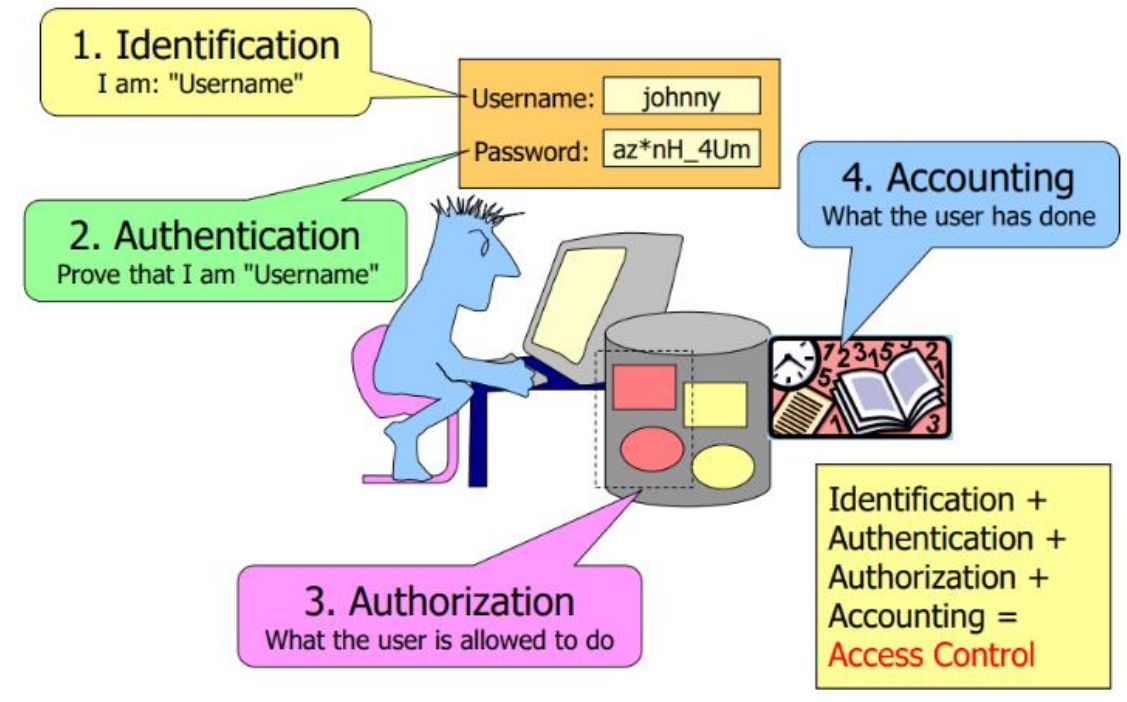
\includegraphics[width=\linewidth]{authentication_flow_diagram.png}

\subsection{Authentication Factors}

\begin{definition}{Authentication Factor Types}\\
    \begin{itemize}
        \item \textbf{Knowledge} Password, PIN, Shared Secret
        \item \textbf{Possession} Smartcard, Token, Mobile, TAN List
        \item \textbf{Biometrics} Fingerprint, Face, Voice
    \end{itemize}
\end{definition}

\subsection{Two factor authentication}

\begin{concept}{Multi-Factor Authentication}\\
    \begin{itemize}
        \item Combination of two methods (Possession, Knowledge, Biometrics)
        \item Considered as strong user authentication
    \end{itemize}
\end{concept}

\subsection{Direct and indirect authentication}

\begin{definition}{Authentication Methods}\\
    \begin{itemize}
        \item \textbf{Direct} Send credentials to server, Server authenticates the user
        \item \textbf{Indirect} Send credentials to server, Handle authentication via authentication server
        
        RADIUS, NTLM, Kerberos, Shibboleth
    \end{itemize}
\end{definition}

\subsection{OTP Generations}

\begin{concept}{OTP Evolution}\\
    \textbf{1st Generation: Increased security}
    \begin{itemize}
        \item Mainly used Possessions (TAN and One-time password tokens)
        \item Vulnerable to e-mail phishing attacks
    \end{itemize}
    
    \textbf{2nd Generation: Prevent E-Mail Phishing}
    \begin{itemize}
        \item Challenge-Response based approach (iTAN, card readers)
        \item Authentication $\rightarrow$ Challenge
        \item Vulnerable to MITM attacks (Online Phishing)
    \end{itemize}
    
    \textbf{3rd Generation: Mobile Phone-based Approach}
    \begin{itemize}
        \item Mobile TAN: Authentication $\rightarrow$ Approve with SMS code
        \item MITM still possible $\rightarrow$ Same security as 2nd Generation
    \end{itemize}
\end{concept}

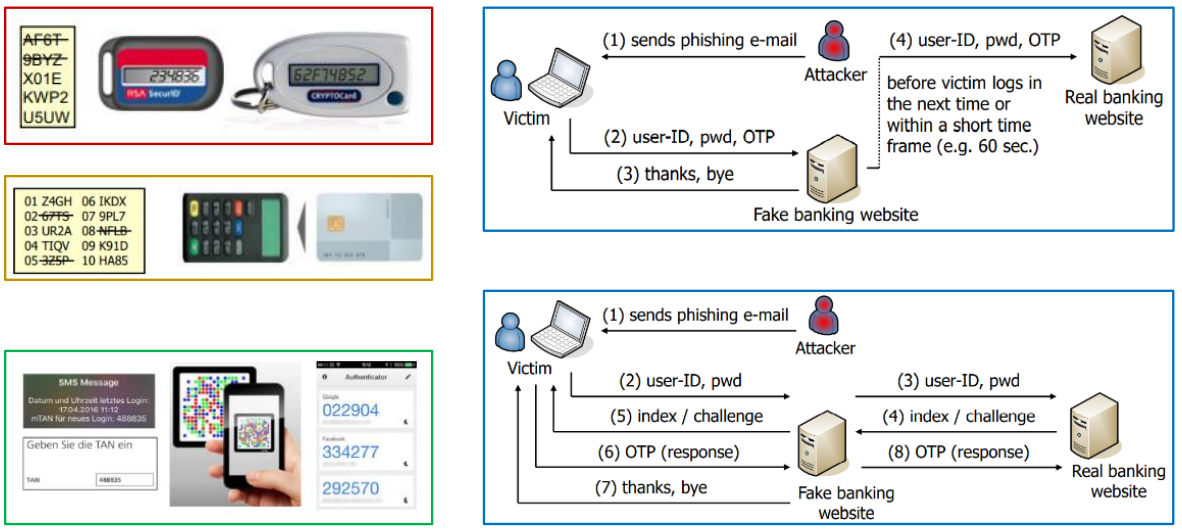
\includegraphics[width=\linewidth]{OTP_generation.png}

\subsection{Windows Domain Authentication}

\begin{definition}{Windows Domain}\\
    A windows domain is a collection of users and services, access is controlled by a Domain Controller (DC). Within a windows domain, we have centralized administration \& SSO.
    \begin{itemize}
        \item One account per user and domain
        \item DC can authenticate users
        \item Credentials need to be entered only once
    \end{itemize}
    
    All users and servers must trust the domain controller.
\end{definition}

\subsection{Windows NT LAN manager (NTLM)}

\begin{concept}{NTLM}\\
    Original authentication protocol in Windows domains.
    \begin{itemize}
        \item Provides "some security" for strong passwords
    \end{itemize}
\end{concept}

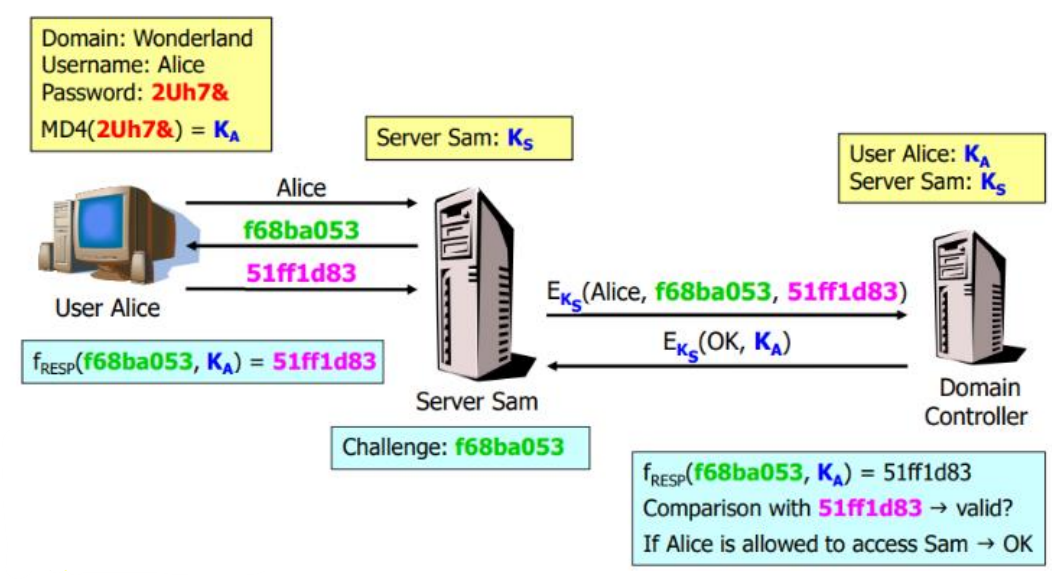
\includegraphics[width=\linewidth]{NTLM_challenge.png}

\subsection{Kerberos (Considered secure)}

\begin{definition}{Kerberos}\\
    Each party
    \begin{itemize}
        \item shares a common secret with a centralised server
        \item trusts the Key Distribution Center (KDC)
    \end{itemize}
    
    \textbf{Properties:}
    \begin{itemize}
        \item Ticket based approach $\rightarrow$ more efficient than NTLM
        \begin{itemize}
            \item Authentication Service
            \item Ticket Granting Service
        \end{itemize}
        \item Prevents replay attacks with timestamps
        \item Weak password $\rightarrow$ offline attacks possible
    \end{itemize}
\end{definition}

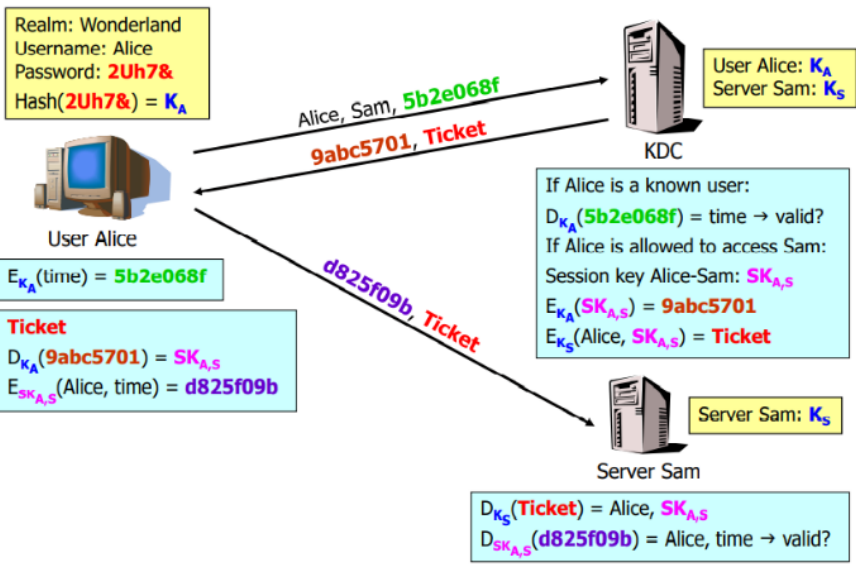
\includegraphics[width=\linewidth]{kerberos.png}

\subsection{Shibboleth (Considered secure)}

\begin{definition}{Shibboleth}\\
    Federated is a system for federated identity management
    \begin{itemize}
        \item Users have one credential that is stored and managed by his home security domain
        \item Components: Organizations, Users, Service providers (SP), Identity providers (IdP)
    \end{itemize}
    
    \textbf{Process:}
    \begin{enumerate}
        \item Connect to Resource (Moodle) Retrieve list of home organizations
        \item Authentication Request Select organization and redirect to Identity Provider
        \item Authentication and Access Enter credentials and access resource
    \end{enumerate}
\end{definition}

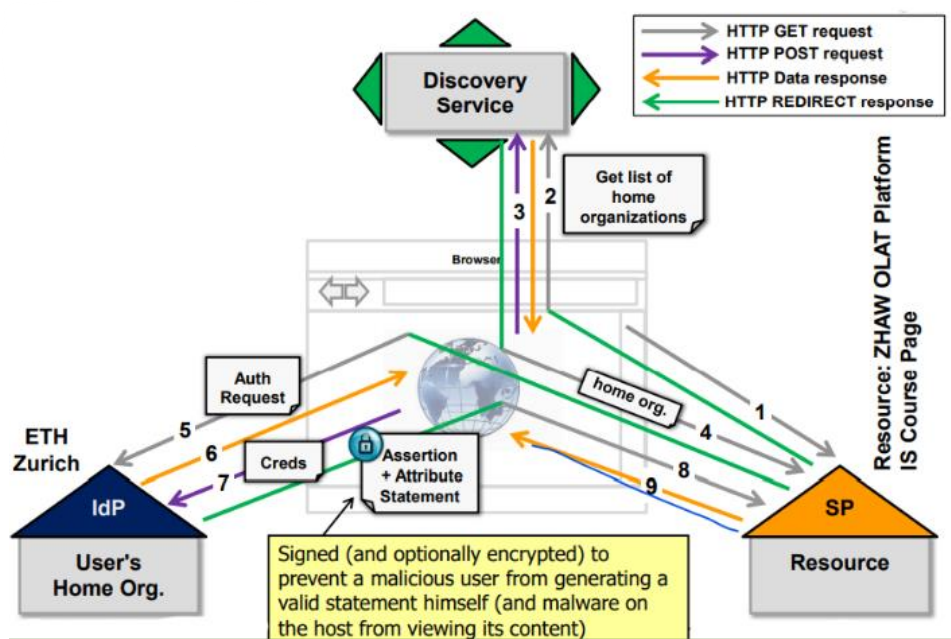
\includegraphics[width=\linewidth]{shibboleth.png}